% This version of CVPR template is provided by Ming-Ming Cheng.
% Please leave an issue if you found a bug:
% https://github.com/MCG-NKU/CVPR_Template.

%\documentclass[review]{cvpr}
\documentclass[final]{cvpr}

\usepackage{times}
\usepackage{epsfig}
\usepackage{graphicx}
\usepackage{amsmath}
\usepackage{amssymb}
\usepackage{indentfirst}
\usepackage{float}
%\usepackage{subfigure}
%\setlength{\parindent}{2em}
% Include other packages here, before hyperref.

% If you comment hyperref and then uncomment it, you should delete
% egpaper.aux before re-running latex.  (Or just hit 'q' on the first latex
% run, let it finish, and you should be clear).
\usepackage[pagebackref=true,breaklinks=true,colorlinks,bookmarks=false]{hyperref}


\def\cvprPaperID{****} % *** Enter the CVPR Paper ID here
\def\confYear{CVPR 2021}
%\setcounter{page}{4321} % For final version only


\begin{document}

%%%%%%%%% TITLE
\title{Human Pose Estimation from a Single Image}

\author{Yikai Wang\\
Student id: 2020233280\\
{}
% For a paper whose authors are all at the same institution,
% omit the following lines up until the closing ``}''.
% Additional authors and addresses can be added with ``\and'',
% just like the second author.
% To save space, use either the email address or home page, not both
\and
Chuanhao Hao\\
Student id: 2020233176\\
{}
}

\maketitle


%%%%%%%%% ABSTRACT
\begin{abstract}
Convolutional networks are powerful visual models that yields hierarchies of features. In this paper, we improve the baselines models for human pose estimation based on ResNet\cite{he2016deep}, we use fully convolutional layers to replace the deconvolutional layers in origin models.
\end{abstract}


\begin{figure*}[h]
\centering
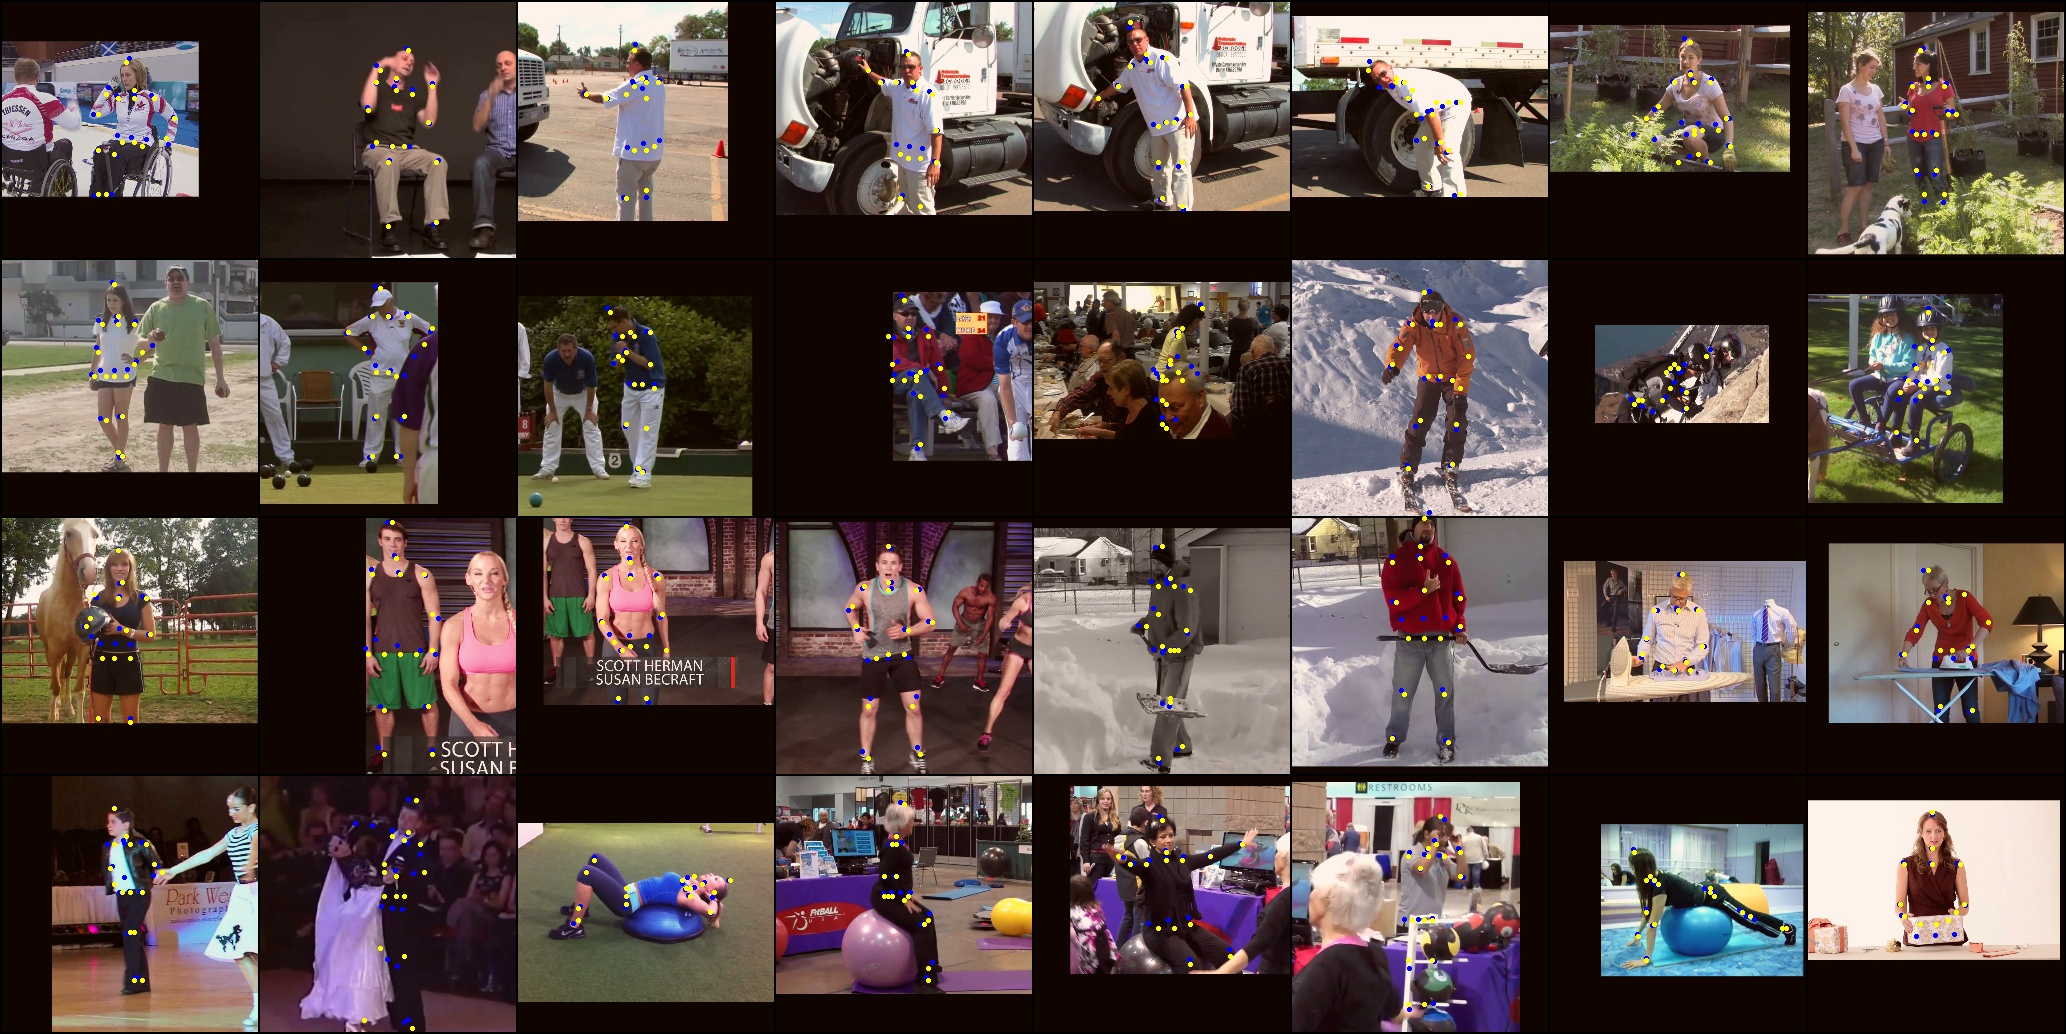
\includegraphics[width=\textwidth]{pred.jpg}
\caption{prediction result of our method}
\end{figure*}

\begin{figure*}[h]
\centering
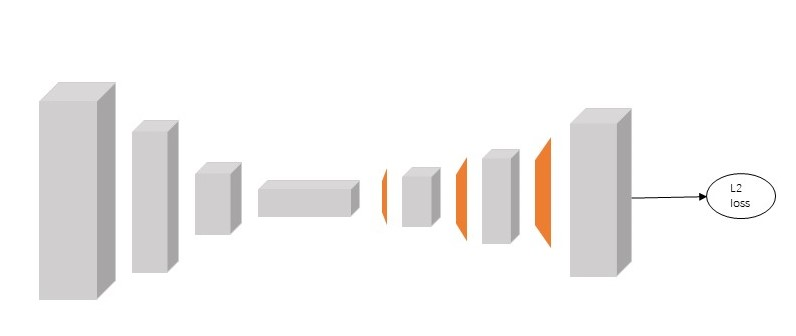
\includegraphics[width=0.7\textwidth]{Resnet.jpg}
\caption{baseline model}
\end{figure*}

\begin{figure*}[h]
\centering
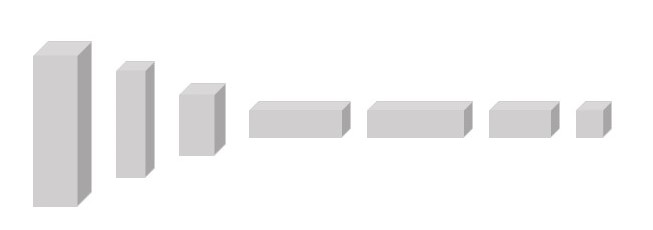
\includegraphics[width=0.7\textwidth]{our method.jpg}
\caption{our method}
\end{figure*}
%%table
\begin{table*}[h]
\begin{center}
\caption{Results on MPII Human Pose(PCKh@0.5)}
\begin{tabular}{c|ccccccc|c}
\hline
&Head&Shoulder&Elbow&Wrist&Hip&Knee& Ankle&Total \\
\hline
Tompson et al.\cite{newell2016stacked}&96.1&91.9&83.9&77.8&80.9&72.3&64.8&82.0\\
Carreira et al\cite{newell2016stacked}. & 95.7&91.7&81.7&72.4&82.8&73.2&66.4&81.3\\
Pishchulin et al.\cite{newell2016stacked}& 94.1&90.2&83.4&77.3&82.6&75.7&68.6&82.4\\
Hu et al.\cite{newell2016stacked}&95.0&91.6&83.0&76.6&81.9&74.5&69.5&82.4\\
Wei et al\cite{newell2016stacked}. &97.8&95.0&88.7&84.0&88.4&82.8&79.4&88.5\\
\hline
\textbf{our model}&\textbf{86.39}&\textbf{65.79}&\textbf{50.01}&\textbf{33.28}&\textbf{50.56}&\textbf{37.64}&\textbf{40.15}&\textbf{52.27}   \\
\hline
\end{tabular}
\end{center}
\end{table*}

\begin{figure*}[h]
\centering
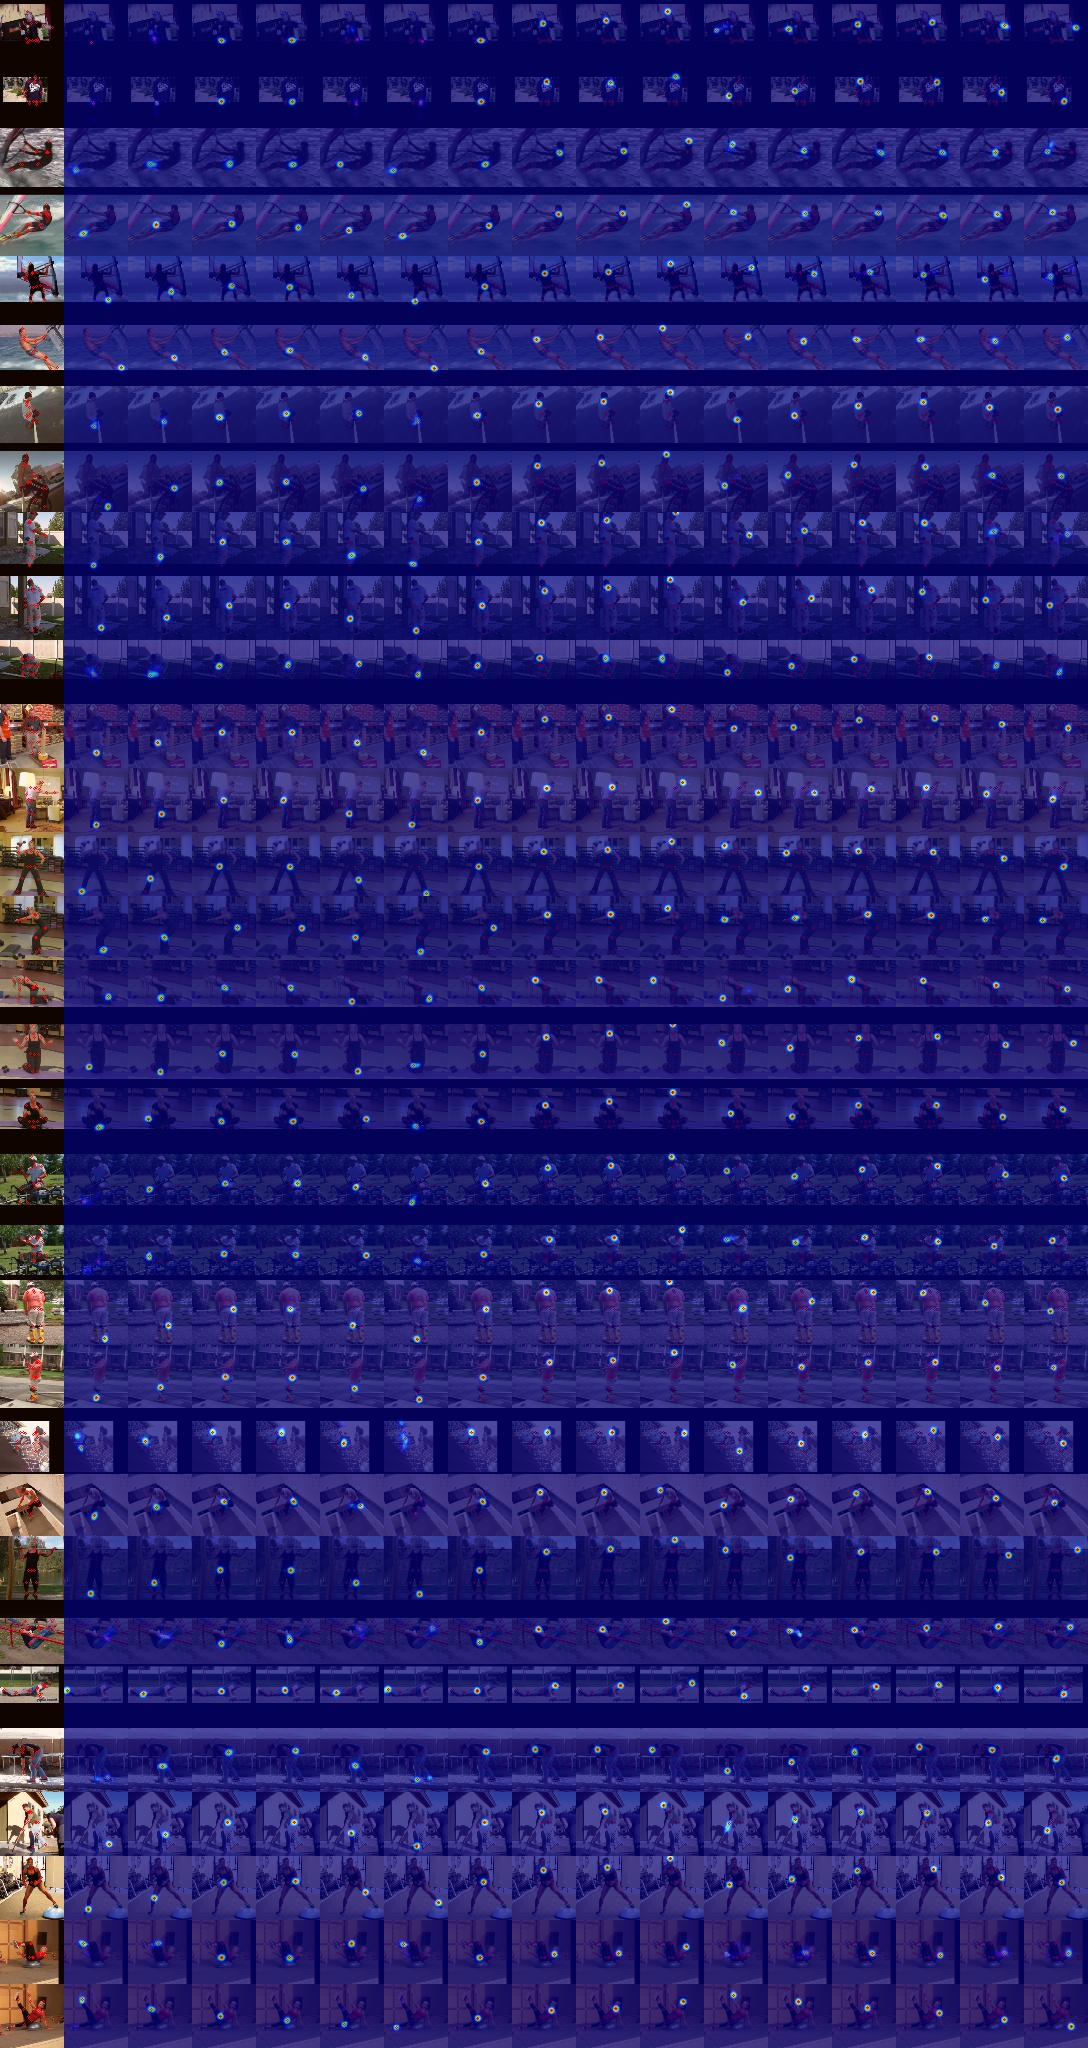
\includegraphics[width=0.6\textwidth]{val_20_hm_pred.jpg}
\caption{Example output produced by our network. On the left we see the final pose estimate provided by the max activations across each heatmap. On the right we show sample heatmaps}
\end{figure*}
%%%%%%%%% BODY TEXT
\section{Introduction}
Human pose estimation, which has been extensively studied in computer vision literature, involves estimating the configuration of human body parts from input data captured by sensors, in particular images and videos. Human pose estimation provides geometric and motion information of the human body which has been applied to a wide range of applications such as human-computer interaction, motion analysis, augmented reality(AR), virtual reality(VR), healthcare,etc. With the rapid development of deep learning solutions in recent years, such solutions have been shown to outperform classical computer vision methods in various tasks including image classification, semantic segmentation and object detection. Significant progress and remarkable performance have already been made by employ deep learning techniques in human pose estimation tasks. However, challenges such as occlusion, insufficient training data, and depth ambiguity still pose difficulties to be overcome. 2D human pose estimation from images and videos with 2D pose annotations is easily achievable and high performance has been reached for the human pose estimation of a single person using deep learning techniques. 2D single-person pose estimation is used to localize human body joint positions when the input is a single-person image. A good human pose estimation system must be robust to occlusion and severe deformation, successful on rare and novel poses, and invariant to challenge in appearance due to factors like clothing and lighting. Early work tackles such difficulties using robust features and sophisticated structured prediction: the former is used to produce local interpretations, whereas the latter is used to infer a globally consistent pose.\\
\indent However, this conventional pipeline has been greatly reshaped by convolutional neural networks\cite{lecun1998gradient}, a main driver behind an explosive rise in performance across many computer vision tasks. Recently pose estimation\cite{tompson2014joint} systems have universally adopted convolutional neural networks as their main building blocks, largely replacing hand-crafted features and graphical models; this strategy has yielded drastic improvements on standard benchmarks. In our project, we utilize the ResNet\cite{he2016deep} to improve the simple baselines for pose estimation\cite{xiao2018simple}, we simplify the base lines method and still achieve a good result.
\section{Related Work}
Traditionally 2D human pose estimation method adopt different hand-crafted feature extraction techniques for body parts, and these early works describe human body as a stick figure to obtain global pose structures. Recently, deep learning-based approaches have achieved a major breakthrough in human pose estimation by improving the performance significantly.\\
\indent Using AlexNet\cite{krizhevsky2017imagenet} as the backbone, Toshev et al\cite{toshev2014deeppose} proposed a cascaded deep neural network regressor named DeepPose, with the introduction of "DeepPose" , research on human pose estimation began shifting from classic approaches to deep learning networks. Toshev et al use their network to directly regress the x,y coordinate of joints. The work by Tompson et al\cite{tompson2014joint} instead generates heatmaps by running an image through multiple resolution banks in parallel to simultaneously capture features at a variety of scales. A critical feature of the method proposed by Tompson et al\cite{tompson2014joint} is the joint use of ConvNet and a graphical model. Their graphical model learns typical spatial relationships between joints. Others have recently tackled this in similar ways\cite{pishchulin2016deepcut} with variation on how to approach unary score generation  and pairwise comparison of adjacent joints. Based on GoogLeNet\cite{szegedy2015going}, Carreira et al.\cite{carreira2016human} proposed an Iterative Error Feedback(IEF) network, which is a self-correcting model to progressively  change an initial solution by injecting the prediction error back to the input space. Sun et al.\cite{sun2017compositional} introduced a structure-aware regression method called  ”compositional  pose  regression”  based  on ResNet-50\cite{he2016deep}. This method adopts a re-parameterized and bone-based representation that contains human body information and pose structure, instead of the traditional joint-based representation. Luvizon et al.\cite{luvizon2019human} proposed an end-to-end regression approach for human pose estimation using soft-argmax function to convert feature maps into joint coordinates in a fully differentiable framework.\\
\indent A good feature that encodes rich pose information is critical for regression-based methods. One popular strategy to learn better feature representation is muti-task learning. By sharing representation between related tasks(eg., pose estimation and pose-based action recognition), the model can generalize better on the original task(pose estimation). Following this direction, Li et al\cite{li2014heterogeneous} proposed a heterogeneous muti-task framework that consists of two tasks: predicting joints coordinates from full images by building a regressor and detecting body parts from image patches using a sliding window. Fan et al.\cite{fan2015combining} proposed a Dual-Source(i.e. images patches and full images) Deep Convolutional Neural Network (DS-CNN) for two tasks: joint detection which determines whether a patch contains a body joint, and joint localization which finds the exact location of the joint in the patch. Each task corresponds to a loss function, and the combination of two tasks leads to improved results. Luvizon et al\cite{luvizon2019human} learned a muti-task network to jointly handle 2D/3D pose estimation and action recognition from video sequences.
\section{Data}
\noindent \textbf{Max Planck Institute for Informatics(MPII) Human Pose Dataset}: This is a popular dataset for evaluation of articulated human pose estimation. The dataset includes around 25000 images containing over 40000 individuals with annotated body joints. The images were systematically collected by a two-level hierarchical method to capture everyday human activities. The entire dataset covers 410 huamn activities and all the images are labeled. Each image was extracted from a YouTube video and provided with preceding and following un-annotated frames. Moreover, rich annotations including body part occlusions, 3D torso and head orientations are also labeled.\\
\textbf{Data Augmentation:} For MPII dataset, it is standard to utilize the scale and center annotations provided with all images. For each sample, these values are used to crop the image around the target person. All input images are then resized to 256$\times$256 pixels. We do data augmentation that includes rotation(+/-30 degrees), and scaling(.75-1.25). We avoid translation augmentation of the image since location of the target person is the critical cue determining who should be annotated by the network.
\section{Methods}
%\begin{figure*}[h]
%\centering
%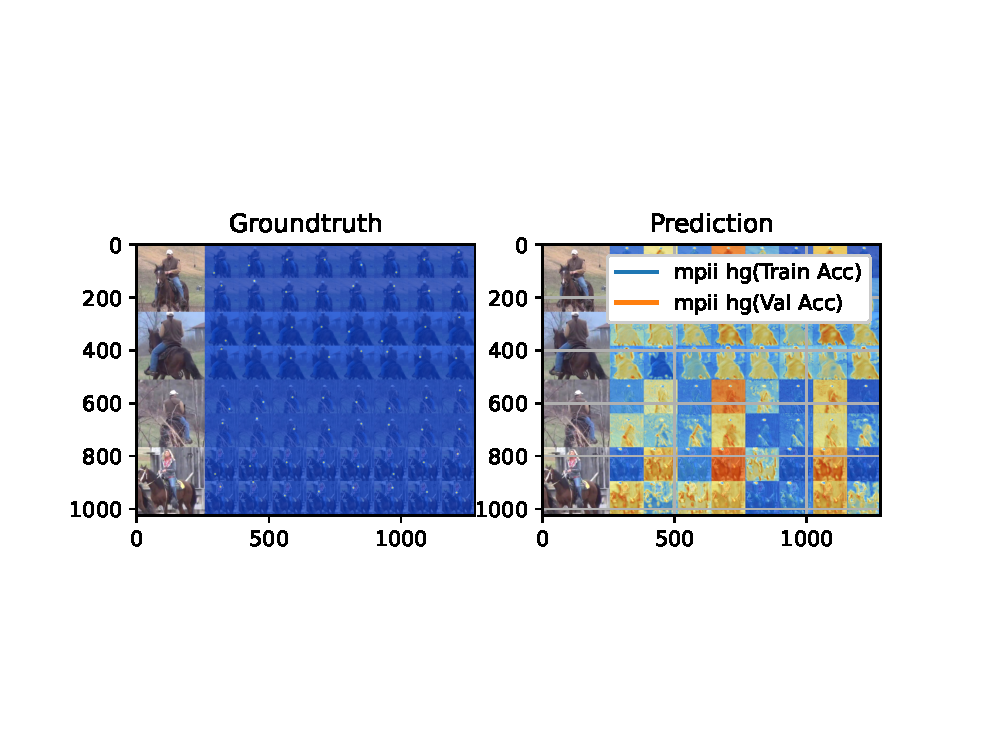
\includegraphics[width=\textwidth]{log.eps}
%\caption{output}
%\end{figure*}
\subsection{Baseline Model}
This section we provided a detail description of the baseline model we use, which is the previous state-of-the-art pose estimation, this model's best results achieves the state-of-the-art at mAP of 73.7 on COCO testdev split, which has an improvement of 1.6\% and 0.7\% over the winner of COCO 2017 keypoint Challenge's single model and their ensembled model. This pose estimation is based on a few deconvolutional layers added on a backone network, ResNet\cite{he2016deep}. It is probably the simplest way to estimate heat maps from deep and low resolution feature maps.\\
\subsubsection{Model Architecture}
This baseline model adds a few deconvolutional layers over the last convolution stage in the ResNet. By default, three deconvolutional layers with batch normalization and ReLU activation are used. Each layer has 256 filters witrh 4$\times$4 kernel. The stride is two, a 1$\times$1 convolutional layer is added at last to generate predicted heatmaps${H_1,\ldots,H_k}$ for all k keypoints. This model combines the upsampling and convolutional parameters into deconvolutional layers without using skip layer connections. Figure.1 shows the architecture of the basline model.
\subsection{Our Method}
ResNet is the most common backbone network for image feature extraction, It is also used for pose estimation. Our method also simply adds a few fully convolutional networks to replace the deconvolutional layers over the last convolution stage in the ResNet, we adopt this structure because it is arguably the simplest to generate heatmaps from deep and low resolution features. \\
\indent Our basic block includes three  convolutional layers, the kernel size are respectively one, three, one. The whole network is set up as follows: Convolutional and max pooling layers are used to process features down to a very low resolution, after reaching the output resolution of the network, three consecutive rounds of 1$\times$1 convolutions are applied to produce the final network predictions. The output of the network is a set of a joint's presence at each and every pixel. Figure.2 shows the architecture of our model, from the image, the left half model is the same as baseline model, the right half of model is different from the baseline model, our model is simpler.
\subsubsection{Fully Convolutional Networks}
Each layer of data in a convet is a three dimension array of size $h\times w\times d$, where $h$ and $w$ are spatial dimension, and $d$ is the feature or channel dimension. The first layer is the image, with pixel size $h\times w$, and $d$ color channels. Location in higher layers correspond to the locations in the image they are path-connected to, which are called they receptive fields.\\
\indent Convets are built on translation invariance. Their basic components(convolution, pooling, and activation functions) operate on local input regions, and depend only on relative spatial coordinates. Writing $x_{i,j}$ for the data vector at location $(i,j)$ in a particular layer, and $y_{i,j}$ for the following layer, these functions compute outputs $y_{i,j}$ by
\[y_{i,j} = f_{ks}({x_{si+\delta i, sj+\delta j}}_{0\leq \delta i,\delta j\leq k)}\]
where $k$ is called the kernel size, s is the stride or the subsampling factor, and $f_{ks}$ determine the layer type: a matrix multiplication or convolution or average pooling, a spatial max for max pooling, or an elementwise nonlinearity for an activation function, and so on for other types of layers.\\
\indent This function form is maintained under composition, with kernel size and  stride obeying the transformation rule
\[ f_{ks}\circ g_{k's'} = (f\circ g)_{k'+(k-1)s',ss'}\]
While a general deep net computes a general nonlinear function, a net with only layers of this form computes a nonlinear filter, which we call a deep filter or fully convolution network. An FCN naturally operates on an input of any size, and produces an output of corresponding(possibly resampled) spatial dimensions.\\
\indent A real-valued loss function composed with FCN defines a task. If the loss function is a sum over the spatial dimensions of the final layer, $l(x,\theta)=\sum l'(x_{ij};\theta)$, its gradient will be a sum over the gradients of each of its spatial components. Thus stochastic gradient descent will be the same as stochastic gradient descent on $l'$, taking all of the final layer receptive fields as a minnibatch.\\
\indent When these receptive fields overlap significantly, both feedforward computation and backpropagation are much more efficient when computed layer-by-layer over an entire image instead of independently patch-by-patch.
\section{Experiments}
\subsection{Training Details}
We evaluate our network on one datasets, MPII Human Pose. It consists of  around 25k images with annotations for multiple people providing 40k  annotated samples(28k training, 11k testing). The test annotations are not provided so in all of our experiments we train on a subset of training images while evaluating on a heldout validating set of around 3000 samples. MPII consists of images taken from a wide range of human activities with a challenge array of widely articulated full-body poses.\indent There are often multiple people visible in a given input image, but without a graphical model or other post processing step the image must convey all necessary information for the network to determine which person deserves the annotation. We deal with this by training the network to exclusively annotate the person in the direct center.\\
\indent The network is trained using Torch and for optimization we use rmsprop with a learning rate of 2.5e-4. We drop the learning rate once by a factor of 5 after validation accuracy plateaus. Batch normalization\cite{ioffe2015batch} is also used to improve training. We also add a batch normalization to every down sample layer. For generating the final test predictions we run both the original input and a flipped version of the image through the network and average the heatmaps together. The final prediction of the network is the max activating location of the heatmap for a given joint.\\
\indent The same techniques as Tompson et al.\cite{tompson2014joint} is used for supervision. A Mean-Square-Error(MSE) loss is applied comparing the predicted heatmap to a ground-truth heatmap consisting of a 2D gaussion(with standard deviation of 1 px) centered on the joint location. To improve performance at high precision thresholds the prediction is offset by a quarter of a pixel in the direction of its next highest neighbor before transforming back to the original coordinate space of the image. In MPII Human Pose, some joints do not have a corresponding ground truth annotation. In these cases the joint is either truncated or severely occluded, so far supervision a ground truth heatmap of all zeros is provided.
\subsection{Results}
Fig.3 shows the prediction result of our method, according to the image, our method can predict the joints approximately. The blue points are our predicted points, the yellow points are the ground truth points.
\subsubsection{Evaluation}
Evaluation is done using the standard Percentage of Correct Keypoints(PCK) metric which reports the percentage of detections that fall within a normalized distance of the ground truth. Table 1 shows the  comparsion with other methods on MPII Human Pose, note that the results in Table 1 are cited from \cite{newell2016stacked} and not implemented by us. Therefore, the performance difference could come from implementation difference. Nevertheless, we believe it is safe to conclude that our baseline has comparable results but is simple.
\section{Conclusions}
In conclusion, our method simplify the baseline model without drop too much accuracy. Due to the limited of computation resource, we do not test more layers and deeper networks, in the future, we may carry out the following ideas:
\begin{enumerate}
\item Apply encoder-decoder layers into our model instead of simple fully connected convolutional layers.
\item Adopt a GAN to train the model which may be better at helping network learn features that are more robust. 
\end{enumerate}


\bibliographystyle{ieee_fullname}
\bibliography{egbib}


\end{document}
